%Importanza della robotica aerea nell'ambito degli interventi di esplorazione e di ispezione di luoghi difficillmente accessibili all'essere umano o pericolosi per esso
%\\Spesso in queste situazioni si preferisce delegare un certo grado di autonomia al robot ed all'occorrenza l'essere umano può intervenire facendo teleoperazione.
%\\Lo scenario pensato è quello di 2 droni, di cui uno deve compiere un task che è stato pensato come peg-in-hole, ad all'interno di un pilone di un ponte, e l'altro deve fornire un punto di vista all'essere umano inquadrando costantemente l'altro drone.
%\\ I droni sono entrambi quadricotteri, per cui sottoattuati per loro natura nello spazio 3D. Per questo motivo il problema viene affrontato nel seguente modo: entrambi i droni prevedono l'utilizzo di PX4 come firmware per la gestione di basso livello; il drone che effettua il task viene controllato in posizione, usando i controllori di bordo standard di PX4; l'altro drone è controllato direttamente in thrust e torque e pianifica in real-time una traiettoria ottima tramite un framework MPC in modo da ottimizzare diversi obiettivi, tenendo conto allo stesso tempo dei vincoli di attuazione del drone. Nel contempo l'operatore umano può effettuare teleoperazione in 2 modi possibili: agendo sul drone che osserva, cambiandone ad esempio il punto di vista dinamicamente, o agendo sul drone che effettua il task, ad esempio proprio per effettuare egli stesso il task di inserzione. 

Nowadays, aerial robotics has become an established tool for operations in hazardous and degraded environments. The use of Unmanned Aerial Vehicles (UAVs) allows for the substitution of human operators in high-risk areas, which is particularly relevant for the inspection and maintenance of aging civil infrastructure. In these scenarios, robotic platforms are deployed to collect data and perform non-destructive measurements, reducing human exposure to dangerous conditions while accessing confined or structurally compromised spaces.
Despite the push towards full autonomy, unstructured real-world environments often require a human-in-the-loop architecture. In such systems, the robot handles low-level stabilization and task execution, while the human operator provides high-level cognitive decision-making skills. To operate effectively, the remote pilot requires a high degree of situational awareness. Relying exclusively on an onboard (egocentric) camera often limits this awareness, especially during close-proximity operations or physical interactions with the environment. This is even more true when having a fixed camera over an underactuated drone. An exocentric point of view, provided by an external observer, maximizes the operator's understanding of the spatial relationship between the interacting robot, the structural constraints, and potential obstacles. Furthermore, to prevent motion sickness and ensure the transmitted video stream is usable for remote decision-making, the observer platform must guarantee smooth and stable camera framing.
\section{Context and Motivations}
\begin{figure}
    \centering
    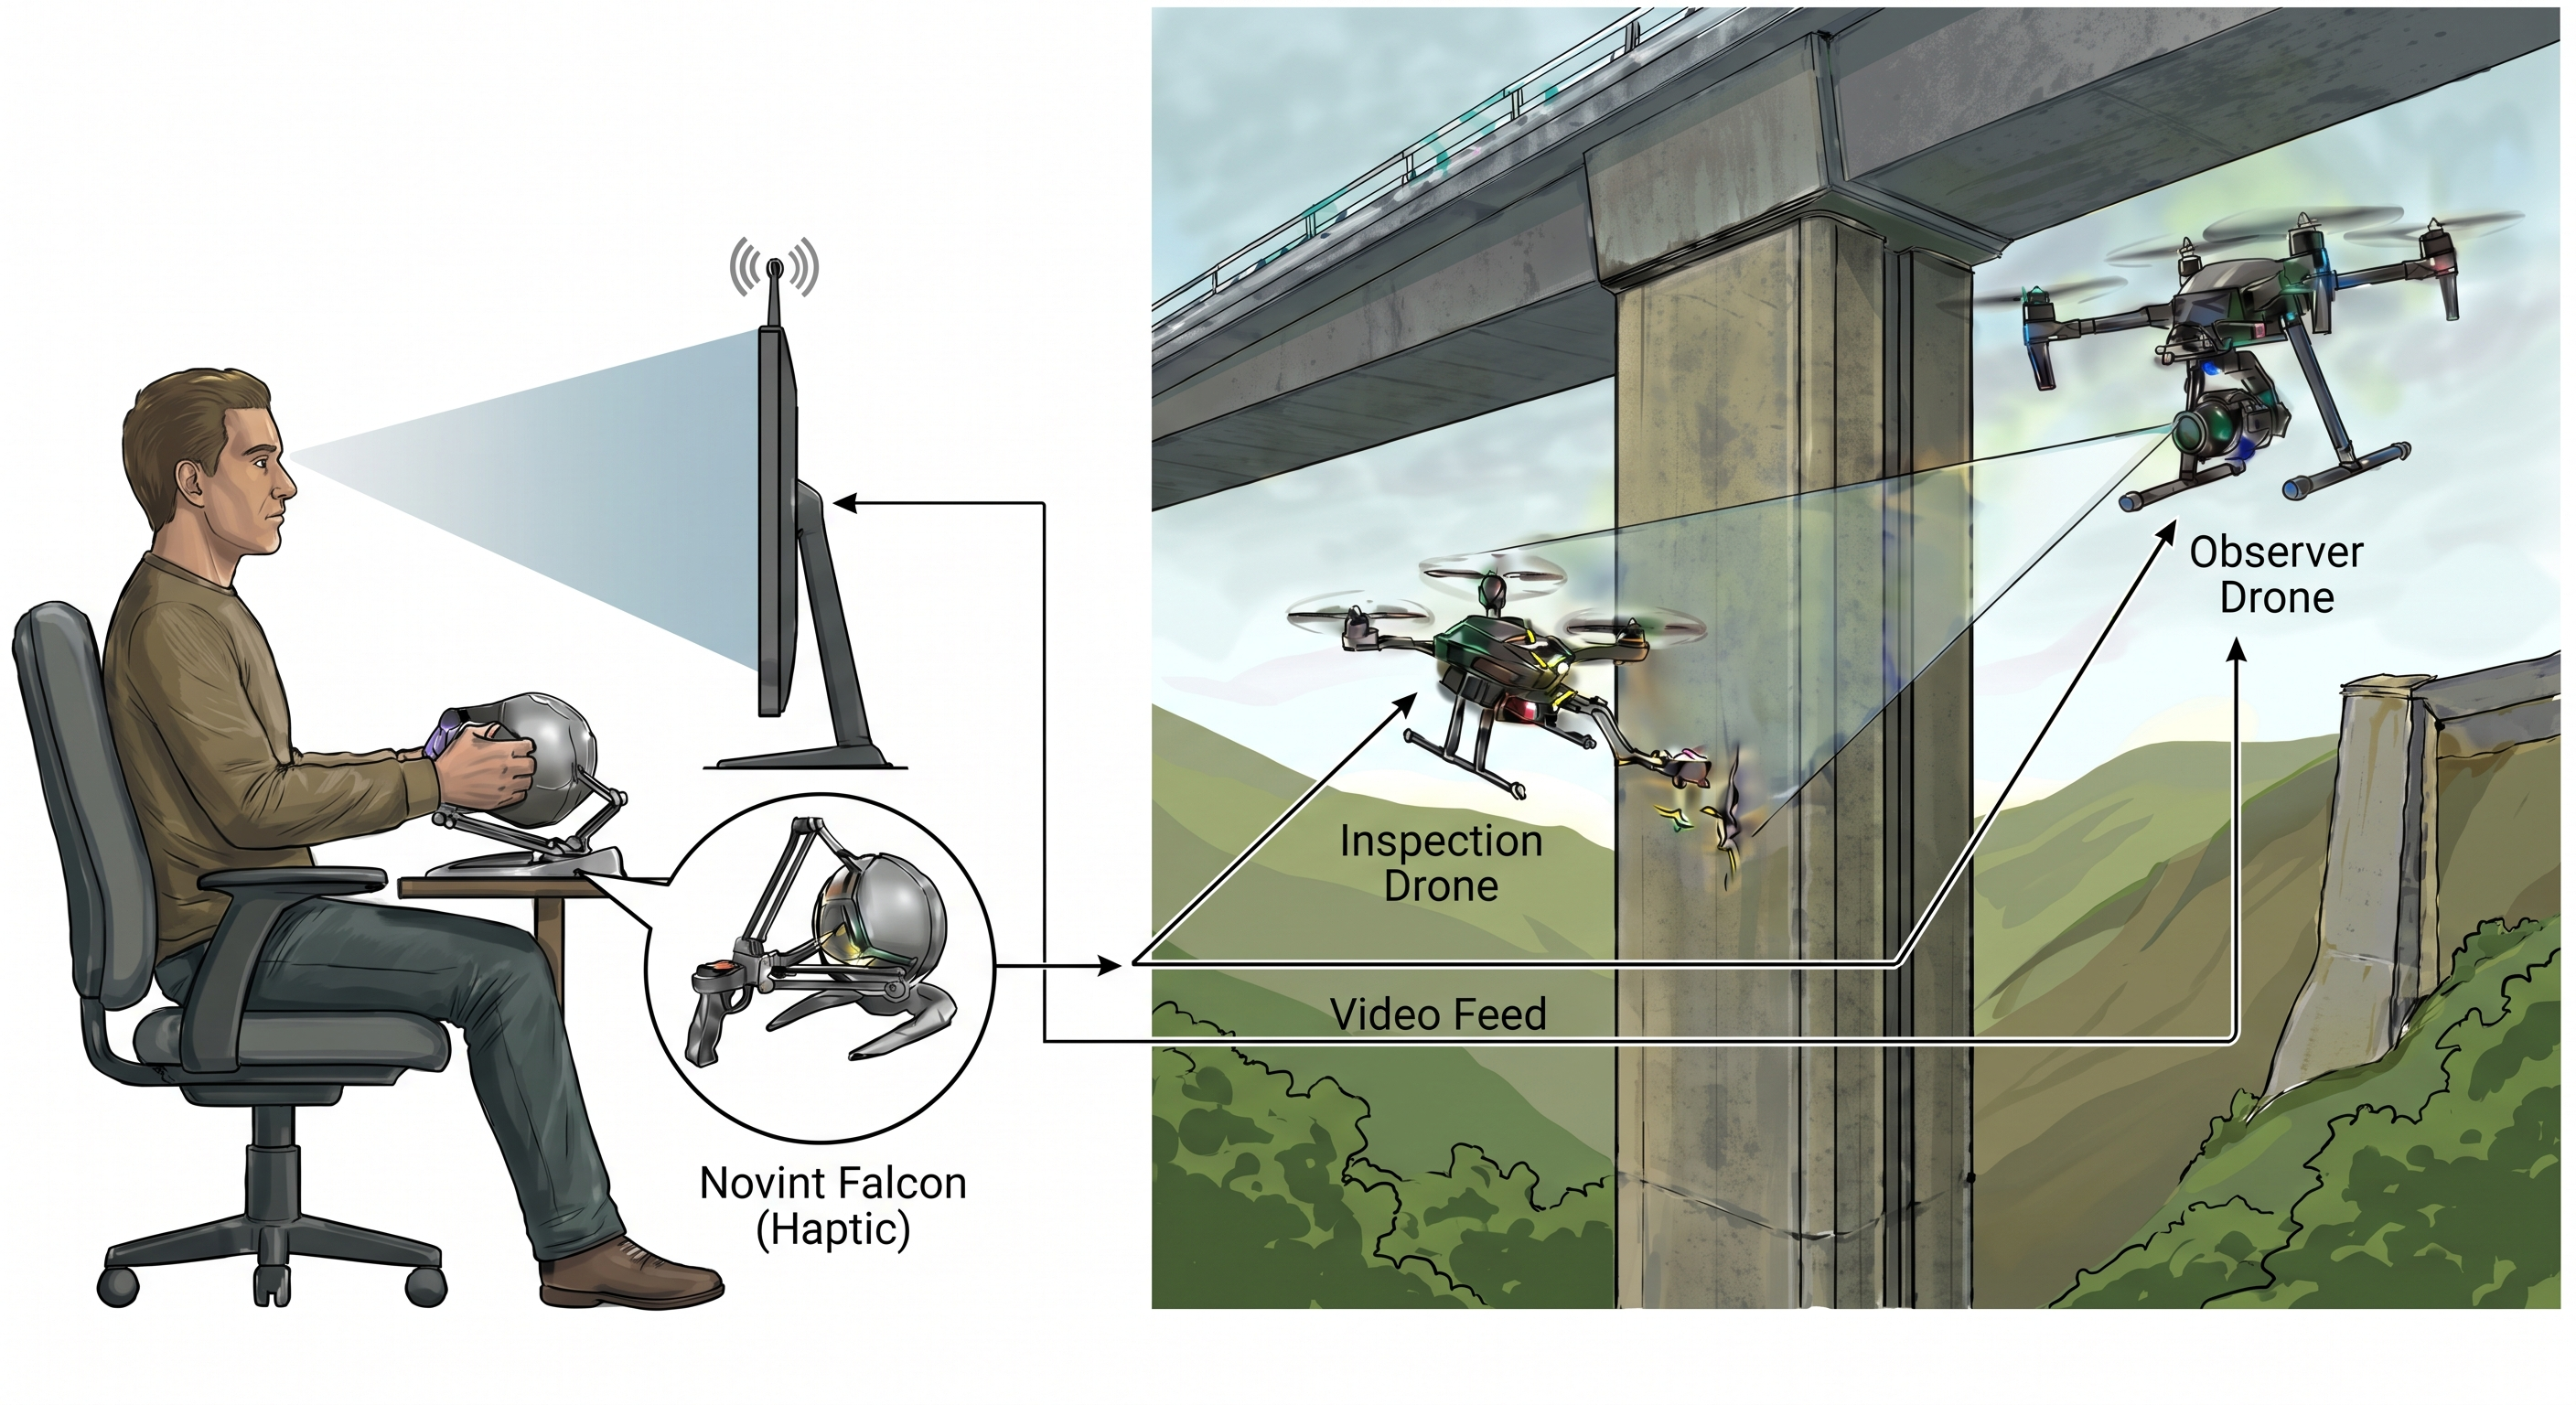
\includegraphics[width=0.8\linewidth]{Immagini/Capitolo1/scenario_introduction.jpeg}
    \caption{Scenario: observer drone frames contact inspection task performed by inspection drone; human operator can command inputs to both drones via haptic device}
    \label{fig:placeholder}
\end{figure}
The thesis addresses a cooperative aerial mission designed for the inspection of confined environments, such as the interior of a bridge pillar. The system relies on a dual-quadrotor setup: an inspection drone tasked with performing a controlled contact with the structure, and an observer drone tasked with providing an optimal exocentric view of the operation.
\\To manage the unpredictability of the environment and the highest precision in inspection contact, a haptic teleoperation interface is integrated into the system, allowing the operator to intervene on two different levels. On one hand, the operator can take command of the observer drone to dynamically change the point of view in the event of occlusions, loss of situational awareness, or unforeseen obstacles. On the other hand, the operator can switch control to the inspection drone to manually guide the final contact phase, compensating for physical uncertainties that the autonomous system cannot resolve.
\section{Contributions}
To support this shared-control paradigm, a multi-layered control and planning framework has been developed.
The core contribution involves the control architecture for the observer UAV, which must satisfy multiple requirements: tracking an unknown and dynamic trajectory of the inspection drone, keeping the target framed, avoiding motion sickness in human operator and responding online to the viewpoint changes commanded by the operator via the haptic device.
To achieve this despite the inherent underactuation of quadrotors, a Nonlinear Model Predictive Control (NMPC) scheme has been designed. The NMPC optimizes the camera framing while ensuring safety by respecting actuation constraints, acting directly at a thrust and torque level and minimizing higher-order time derivatives in the cost function. Moreover, to compensate for external disturbances and model mismatches, a MBE (Momentum Based Estimator) is updated online, making the control intrinsically robust.
\\On the other hand, the inspection UAV operates using a position control strategy modified with an admittance filter to ensure a stable execution of the physical contact.
\\Human is inserted inside the loop through bilateral teleoperation over NMPC observer UAV and unilateral teleoperation to the interacting one, bringing the framework into Shared Control.
\\Everything is orchestrated by a FSM that decides which are the best views for the human according to FSM state and handles emergencies.
\\To guarantee system reliability and facilitate a realistic transition to hardware, the entire high-level control architecture for both platforms has been integrated with the standard and open-source \texttt{PX4} autopilot firmware.

\section{Thesis Outline}
The here presented thesis  is structured as follows. 
Chapter 2 reviews the state of the art concerning shared control architectures, vision modalities in teleoperation, and online planning and control methods for aerial robotics. 
Chapter 3 defines the problem statement and presents an overview of the proposed dual-UAV system architecture, detailing the exocentric vision paradigm, the contact inspection requirements, and the sequential phases of the cooperative mission. 
Chapter 4 provides the mathematical formulation of the problem. It details the rigid body dynamics of the quadrotors, the Non-linear Model Predictive Control (NMPC) framework designed for the observer drone's visual tracking, the human-robot shared control layer, together with the mathematical generation of haptic references and the Artificial Potential Fields (APF) used to render the force feedback to the operator and the admittance control scheme utilized by the inspection drone to manage physical interactions. 
Chapter 5 describes the software and hardware implementation of the overall framework. It covers the ROS 2 middleware integration, the PX4 flight stack interactions, the finite state machine governing the mission supervisor, and the real-time execution details of the NMPC and admittance nodes. 
Chapter 6 presents the simulation and experimental results, validating the control framework's performance, the tracking accuracy, and the effectiveness of the haptic shared control paradigm. 
Finally, Chapter 7 summarizes the conclusions of this work and outlines potential directions for future research.   